\documentclass[9pt,twocolumn]{article}

\usepackage[letterpaper,margin=0.65in,columnsep=0.24in]{geometry}
\usepackage[T1]{fontenc}
\usepackage[utf8]{inputenc}
\usepackage{lmodern}
\usepackage{microtype}
\usepackage{amsmath,amssymb}
\usepackage{graphicx}
\usepackage{booktabs}
\usepackage{array}
\usepackage{xcolor}
\usepackage{xurl}
\usepackage[numbers,sort&compress]{natbib}
\usepackage[colorlinks=true,linkcolor=blue!55!black,citecolor=blue!55!black,urlcolor=blue!55!black]{hyperref}
\usepackage[font=small,labelfont=bf]{caption}

\setlength{\parindent}{1em}
\setlength{\parskip}{0pt}
\setlength{\bibsep}{0pt}
\newcommand{\system}{Open Agronomy Agent}
\IfFileExists{generated_results.tex}{\newcommand{\RCObservations}{8,676}
\newcommand{\RCTrials}{nine}
\newcommand{\RCScoredCases}{49/241}
\newcommand{\RCSemanticJudgments}{zero}
\newcommand{\RCRetrievalSource}{22/26}
\newcommand{\RCRetrievalPattern}{46/50}
\newcommand{\RCFieldAdmitted}{11/16}
\newcommand{\RCCanonicalCalc}{14/16}
\newcommand{\RCToolAudit}{16/16}
\newcommand{\RCLunaCalls}{2,841}
\newcommand{\RCLunaTokens}{10,919,444}
\newcommand{\RCLunaCost}{\$3.0463}
}{
  \newcommand{\RCObservations}{pending}
  \newcommand{\RCTrials}{pending}
  \newcommand{\RCScoredCases}{pending}
  \newcommand{\RCSemanticJudgments}{pending}
  \newcommand{\RCRetrievalSource}{pending}
  \newcommand{\RCRetrievalPattern}{pending}
  \newcommand{\RCFieldAdmitted}{pending}
  \newcommand{\RCCanonicalCalc}{pending}
  \newcommand{\RCToolAudit}{pending}
  \newcommand{\RCLunaCalls}{pending}
  \newcommand{\RCLunaTokens}{pending}
  \newcommand{\RCLunaCost}{pending}
}

\title{What RC3 Measured:\\A Reproducible Harness Checkpoint for an Evidence-Governed Agronomy Agent}
\author{Tyler Knecht}
\date{15 August 2026}

\begin{document}
\raggedbottom
\maketitle

\begin{abstract}
Evaluation of an evidence-governed agent must test more than its language model: routing, retrieval, authority policy, deterministic tools, answerability decisions, verification, retention, and analysis boundaries can dominate the final response. We report RC3, an exposed, nonclaim development regression for \system{}. Three candidate-system configurations were executed in three repeated trials across four arms and 241 project-authored Canadian cases, producing \RCObservations{} receipt-bound observations. The full matrix and nine content-addressed retention bundles passed structural and lineage audits. However, only \RCScoredCases{} cases per arm have a defined deterministic endpoint, and the run contains \RCSemanticJudgments{} automated or human semantic judgments. The frozen full-system calculation parser accepted \RCCanonicalCalc{} cases; a post-run audit found all \RCToolAudit{} typed tool payloads within numeric tolerance, exposing a unit-alias defect without rewriting the frozen result. Expected retrieval sources appeared in \RCRetrievalSource{} positive cases and \RCRetrievalPattern{} required patterns were present. Full-system behavior included deterministic holds, tool results, clarifications, and extensive answer verification, demonstrating harness reachability but not answer correctness. RC3 therefore supports a reproducible harness checkpoint and a concrete repair agenda, not a model ranking, agronomic reliability claim, or Benchmark v3 result.
\end{abstract}

\section{Introduction}

Agronomic answers are situated decisions. Crop, stage, field history, measurements, jurisdiction, authority currency, and the consequence of error all matter. A language model does not by itself establish field conditions or current legal-label authority. \system{} addresses this problem by treating the generator as one replaceable component inside a governed pipeline: a stable instruction kernel, structured field context, policy-admitted retrieval, graph context, typed calculations, evidence-sensitive answerability, verification, and durable trace receipts.

Retrieval-augmented generation can condition generation on retrieved passages \citep{lewis2020rag}; the SoilWise v0.2.3 artifact organizes soil-health concepts and relations using SKOS and linked vocabularies \citep{soilwisekg2025}; and MLX provides a machine-learning framework for Apple-silicon systems \citep{mlxframework}. These capabilities do not by themselves establish answer quality, privacy, or disconnected operation. Motivated by research on appropriate reliance on imperfect automation \citep{lee2004trust}, \system{} makes evidence and authority boundaries observable and calibrates intervention. The evaluation problem is therefore twofold: compare candidate-system behavior while also testing whether the harness exposes, binds, and survives its own failures.

This paper reports the completed RC3 development round as a checkpoint. It supersedes the earlier RC1 interpretation without rewriting it. The central question is not ``which model won?'' It is: \emph{what did the frozen experiment actually measure, what did the harness demonstrably execute, and what evidence is still absent?}

\section{System and release boundary}

The evaluated runtime uses an immutable Canadian offline master with 969 rows from 20 admitted sources, augmented by project boundary material, SoilWise-derived context, a compact NRCS analogy pack, and two manifest-bound graphs. Policy roles physically separate context-only rows from material requiring live authority. Current product labels, regulations, weather, and field measurements remain external authorities; absence is surfaced rather than inferred.

The full-system request path routes the question, compiles supplied field context, retrieves documents and graph nodes, plans typed capabilities, checks evidence sufficiency, chooses an answerability action, generates or returns a deterministic result, verifies the draft when configured, and persists a staged provenance graph. The remote Luna path additionally uses an exact, recipient-bound egress contract with case, prompt, corpus-row, graph-node, and authorization membership. Private overlays were disabled. These controls constrain the evaluation transport; they do not promote the resulting answers.

RC3 was executed from source commit \texttt{3e30fb5d} and benchmark-source snapshot \texttt{25fb45e1...6c273c3}. The accompanying release candidate's validation receipt binds the file identities of later successor repairs; none is part of the measured system.

\section{Experimental design}

\subsection{Cases, arms, and candidate configurations}

The frozen suite contains 241 project-authored cases in six lanes: 90 Canadian decision-quality, 31 advisory-transfer, 32 field-history-lineage, 39 official-source-boundary, 33 retrieval-lineage, and 16 objective calculation cases. It contains no verified real-user questions. The suite is public, exposed, and was used during system tuning; it cannot estimate prospective generalization.

Each candidate configuration was evaluated in four ordered arms:

\begin{enumerate}
  \item \textit{raw model}: the question only;
  \item \textit{kernel}: stable instruction and answer contract;
  \item \textit{kernel + field}: the same kernel plus synthetic structured field context; and
  \item \textit{full system}: the configured retrieval, graph, tool, authority, answerability, verification, and postprocessing bundle.
\end{enumerate}

The candidates were a 4-bit Gemma 3 270M configuration, a 4-bit Gemma 4 E2B configuration, and Luna High at high reasoning effort. They are not pure model comparisons: the full-system verifier profiles were respectively constrained, balanced, and frontier, and maximum generation settings differed. Adjacent arm contrasts identify bundle changes, not individual component effects.

Three fresh-process trials used distinct case-order and declared local generation seeds. The local profiles resolved temperature zero to argmax and produced identical bytes across trials. Luna does not expose a configurable seed through this transport. We therefore call all nine executions repeated trials, not independent stochastic samples.

\subsection{Outcome authority}

Figure~\ref{fig:coverage} states the most important boundary. The 16 calculation cases have an objective numeric/unit/tolerance scorer. Thirty-three official-source cases have a frozen lexical contract; six cases in that lane do not. The lexical proxy measures required and forbidden text-pattern coverage and is useful only for regression diagnostics. It is not semantic correctness. The remaining 192 cases per arm require trace interpretation or independent human review.

Each trial contains a two-phase blinded packet for 90 raw/full decision-quality pairs, but no reviewer responses were populated. No automated semantic judge was run. This avoids granting an LLM judge promotion authority amid documented position, verbosity, limited-reasoning, and---in some models---self-preference risks \citep{zheng2023judge,wataoka2024selfpreference}; it also leaves RC3 unable to rank agronomic answer quality.

\begin{figure*}[t]
  \centering
  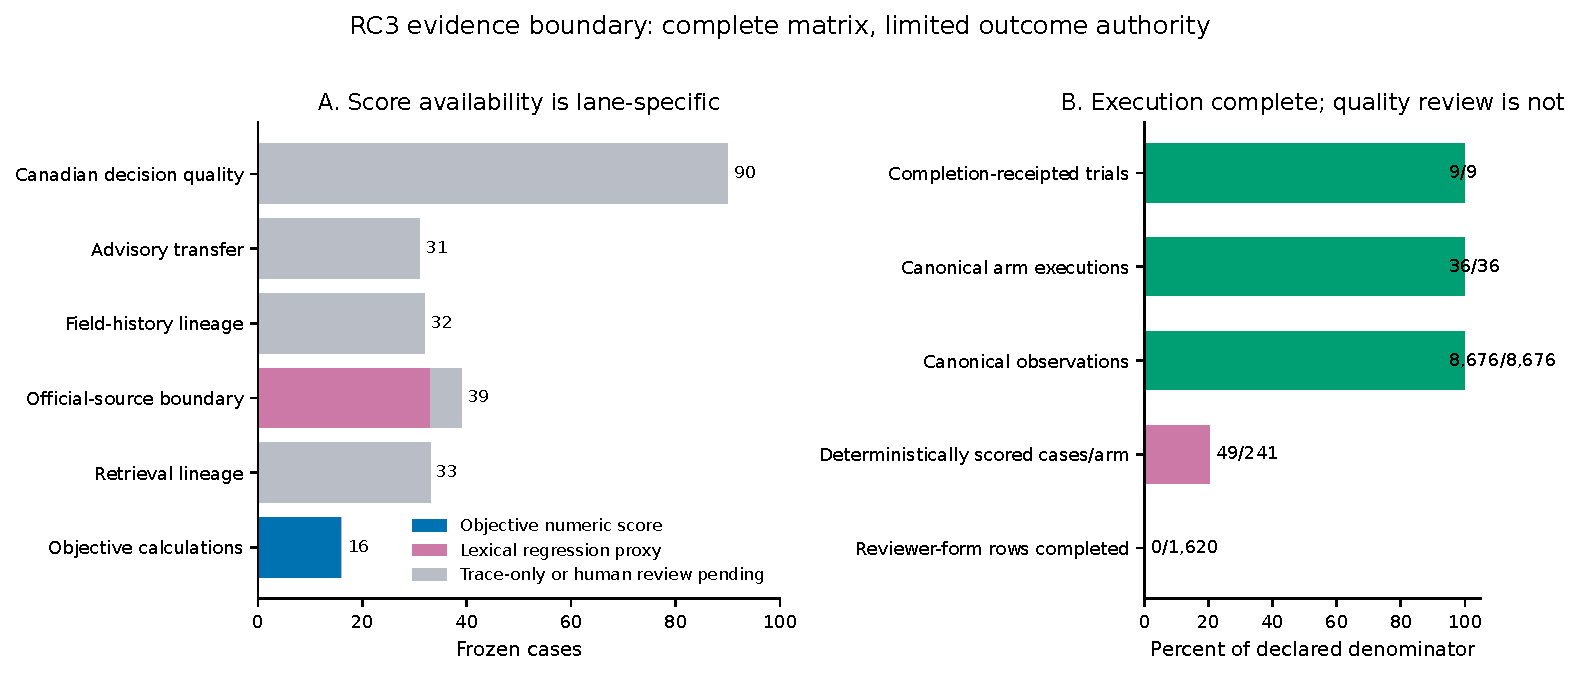
\includegraphics[width=0.98\textwidth]{figures/rc3_evidence_coverage.pdf}
  \caption{\textbf{Evidence availability and completion.} The 3-by-3-by-4-by-241 execution matrix is complete and retention-bound, but deterministic outcomes exist for only 49 cases per arm. Trace presence and blank review packets are not substitute scores.}
  \label{fig:coverage}
\end{figure*}

\subsection{Estimands and sensitivity intervals}

Let $y_{m,a,i,t}$ be a defined endpoint for candidate configuration $m$, arm $a$, case $i$, and trial $t$. Trials are averaged within case before the finite-suite mean:
\begin{equation}
\bar y_{m,a,i}=\frac{1}{3}\sum_{t=1}^{3}y_{m,a,i,t},\qquad
\hat\mu_{m,a}=\frac{1}{N}\sum_{i=1}^{N}\bar y_{m,a,i}.
\end{equation}
Paired arm contrasts average within-case differences. Plotted intervals use 50,000 case resamples of trial-averaged values, sharing resample indices across candidate and arm cells within each metric family; the base seed is 20260815 with deterministic metric-family offsets. Arm contrasts resample paired within-case differences. These are fixed-suite composition sensitivity intervals, not population or human-agreement confidence intervals. We report no $p$ values, significance tests, equivalence claims, or composite score. The historical v2 preregistration specified engineering margins for different estimands, but exact-case exposure invalidated it as an untouched evaluation, and it defines neither promotion margins nor a multiplicity family for the RC3 endpoints analyzed here.

\section{Results}

\subsection{Execution and retention integrity}

All \RCTrials{} candidate-trial commands completed four 241-row arms. The 36 execution IDs and all 8,676 observation IDs are unique. Each of 2,169 matched trial keys has exactly four arm observations. Final JSONL files equal their completed partial files byte-for-byte; all nine SQLite databases pass integrity and foreign-key checks; and their live hashes match the completion-referenced retention manifests. No automated semantic judge was requested or run; judge-related database tables contain zero rows, and no automated-judge output artifacts are present. These findings establish a coherent measurement substrate, not the validity of a response.

\subsection{Deterministic endpoints}

Table~\ref{tab:metrics} and Figure~\ref{fig:metrics} retain all three observed trial means. The full-system objective score is 87.5\% for every configuration because the same deterministic calculator path handled all 16 cases. Two case identities, repeated across every candidate-trial, were numerically correct but rejected by the frozen parser: \texttt{ca\_calc\_map\_04} returned 86.538~kg product/ha and \texttt{ca\_calc\_urea\_03} returned 217.391~kg product/ha. Both lie inside their reference tolerances, but the generic product-mass unit was absent from the product-specific alias contracts. The canonical result remains 14/16. The separately marked 16/16 result is a post-run typed-payload audit and does not rewrite RC3.

The official-source lexical proxy is defined on 33 cases. Its values can reveal prompt or fallback text-contract changes, but a higher value cannot establish a better agronomic answer. In particular, the Luna full-system proxy is lower than its kernel-plus-field value; the metric cannot determine whether this reflects safer compression, lost useful detail, or lower semantic quality. Human review is required to discriminate those explanations.

\begin{figure*}[t]
  \centering
  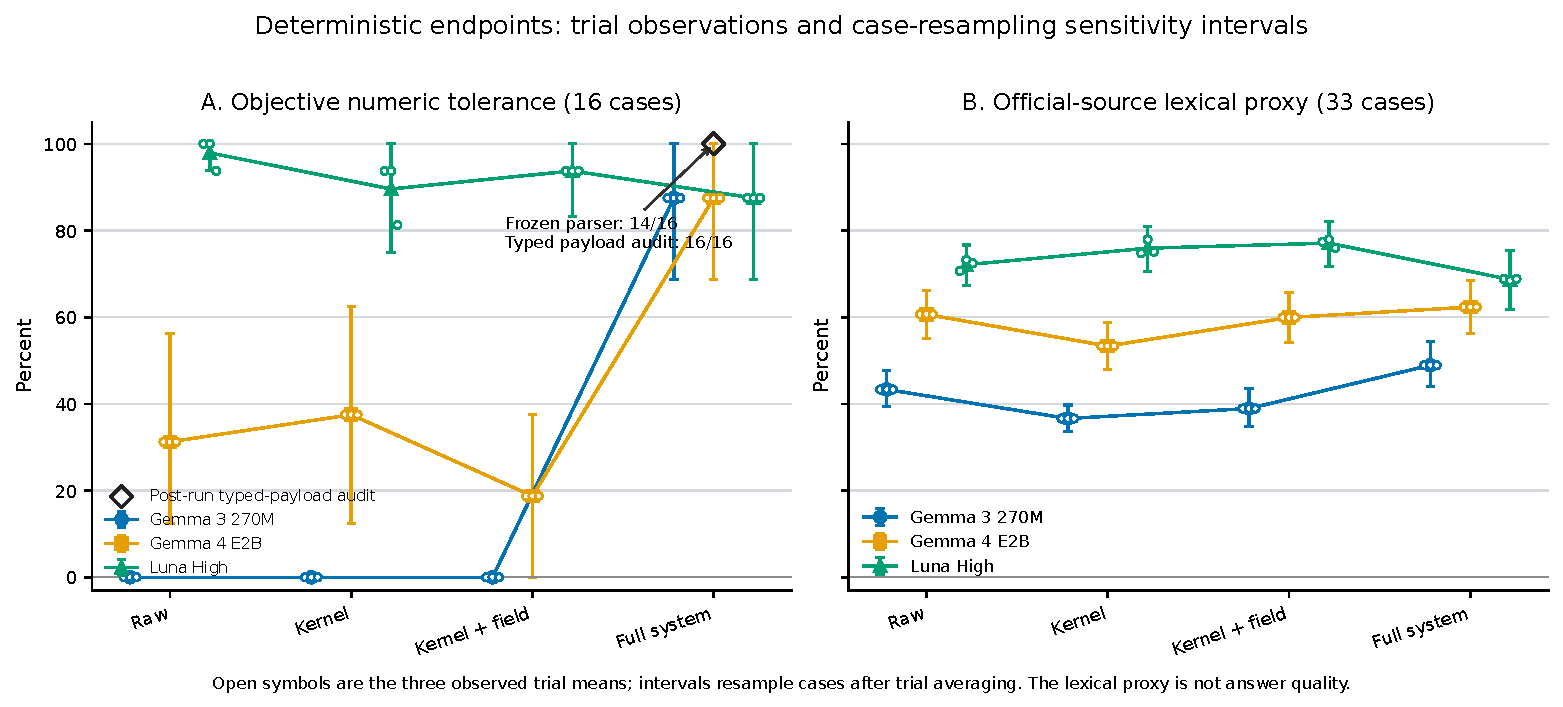
\includegraphics[width=0.98\textwidth]{figures/rc3_deterministic_metrics.pdf}
  \caption{\textbf{Defined deterministic endpoints.} Filled marks are case-level finite-suite means; small open marks are the three observed trial means; whiskers are case-resampling sensitivity intervals with shared draws within each metric family. The open diamond is the explicitly post-run typed-payload calculation audit. The lexical panel is a regression proxy, not answer quality.}
  \label{fig:metrics}
\end{figure*}

\begin{table*}[t]
\centering
\caption{Deterministic development metrics. Values are finite-suite means across case-level trial averages. The official-source metric is a lexical contract regression, not answer quality.}
\label{tab:metrics}
\small
\begin{tabular}{llrrrr}
\toprule
Candidate configuration & Metric & Raw & Kernel & Kernel + field & Full system \\
\midrule
Gemma 3 270M & Numeric tolerance (\%) & 0.00 & 0.00 & 0.00 & 87.50 \\
Gemma 3 270M & Lexical proxy (\%) & 43.33 & 36.63 & 38.94 & 48.91 \\
Gemma 4 E2B & Numeric tolerance (\%) & 31.25 & 37.50 & 18.75 & 87.50 \\
Gemma 4 E2B & Lexical proxy (\%) & 60.65 & 53.36 & 59.93 & 62.34 \\
Luna High & Numeric tolerance (\%) & 97.92 & 89.58 & 93.75 & 87.50 \\
Luna High & Lexical proxy (\%) & 72.11 & 75.92 & 77.10 & 68.69 \\
\bottomrule
\end{tabular}
\end{table*}

\begin{table}[t]
\centering
\caption{Full-system harness activation across three trials per configuration. Counts are execution traces, not correctness scores.}
\label{tab:harness}
\small
\begin{tabular}{lrrr}
\toprule
Configuration & Generated & Holds & Verifier triggered \\
\midrule
Gemma 3 & 489 & 174 & 453 \\
Gemma 4 & 489 & 174 & 333 \\
Luna & 489 & 174 & 296 \\
\bottomrule
\end{tabular}
\end{table}


\subsection{Retrieval, tools, holds, and verification}

Full-system output origin is identical in count across configurations: per trial, 163 paths generated a model draft, 16 returned a typed deterministic tool result, 58 returned an evidence-sufficiency hold, and 4 requested missing calculator input. Thirty-one of 90 decision-quality cases ended in deterministic holds. Consequently, a full-system response is often a harness result rather than a direct sample of generator capability.

Retrieval was likewise invariant before generation. Documents were present on 207/241 cases and graph nodes on 176/241. Reconstructing source expectations from the frozen source-suite lineage, \RCRetrievalSource{} positive retrieval cases surfaced their named source; 13/16 cases satisfied every required pattern and \RCRetrievalPattern{} individual patterns were present. For field-history lineage, \RCFieldAdmitted{} expectations whose source exists in the current Canadian master were retrieved. Thirteen cases reference intentionally unadmitted sources and had zero leakage. Twenty-nine prospective decision-card IDs across 28 cases are absent from runtime and are not scored as graph misses.

Verifier behavior differs by candidate configuration. Across three full-system trials, verification was triggered on 453 Gemma 3, 333 Gemma 4, and 296 Luna responses. Gemma 3 used 453 fallback/degraded results and accepted no rewrite; Gemma 4 used 273 fallbacks and 45 accepted rewrites; Luna used 181 fallbacks and 106 accepted rewrites. Without blinded draft-versus-final review, these counts show reachability and containment, not improvement.

\begin{figure*}[t]
  \centering
  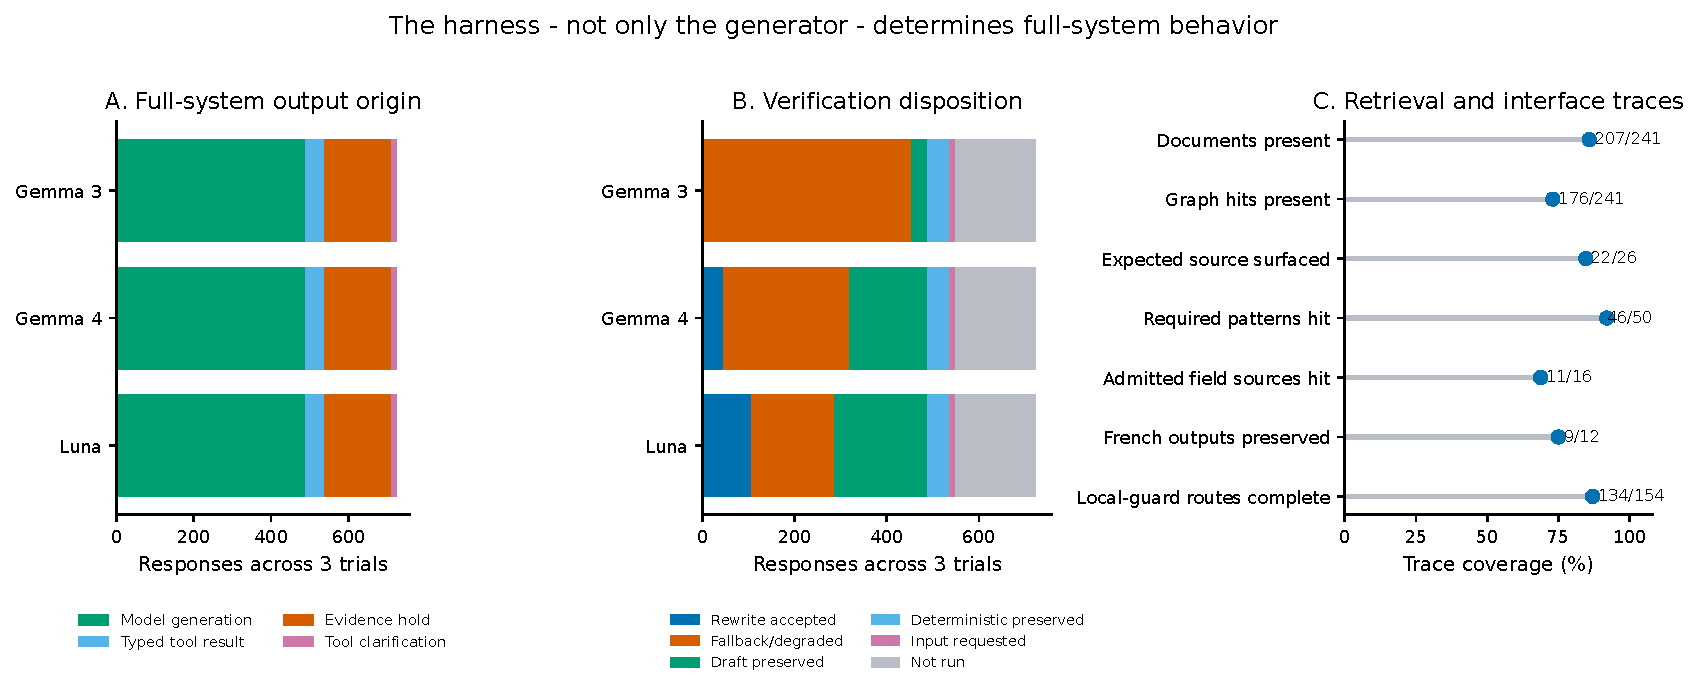
\includegraphics[width=0.99\textwidth]{figures/rc3_harness_behavior.pdf}
  \caption{\textbf{Harness behavior.} Output origin and verifier disposition cover all 723 full-system responses per candidate. Retrieval and interface ratios use one invariant trial's case denominator where execution precedes the generator. None is an answer-quality score.}
  \label{fig:harness}
\end{figure*}

\subsection{Repeatability and resource observations}

Both local MLX configurations were byte-identical across all three trials for every arm. This is useful fresh-process and order repeatability under temperature-zero argmax, but it supplies no independent sampling variance. Luna varied on most raw, kernel, and field cases; the full system was exact on 123/241 cases, largely because deterministic holds, tool results, clarifications, and shared fallbacks constrain outputs.

Latency is reported descriptively as medians and p95 values. Sequential arm order, backend differences, model warmth, and deterministic bypasses prevent causal speed comparison. One Gemma 4 kernel observation recorded 5,062.879 seconds; the unexplained host/runtime stall is preserved and shown rather than winsorized. Luna recorded \RCLunaCalls{} candidate and answer-verifier calls, \RCLunaTokens{} total tokens, and an API-equivalent estimate of \RCLunaCost{}. Actual ChatGPT-authenticated billing and local energy use were not observed.

\begin{figure*}[t]
  \centering
  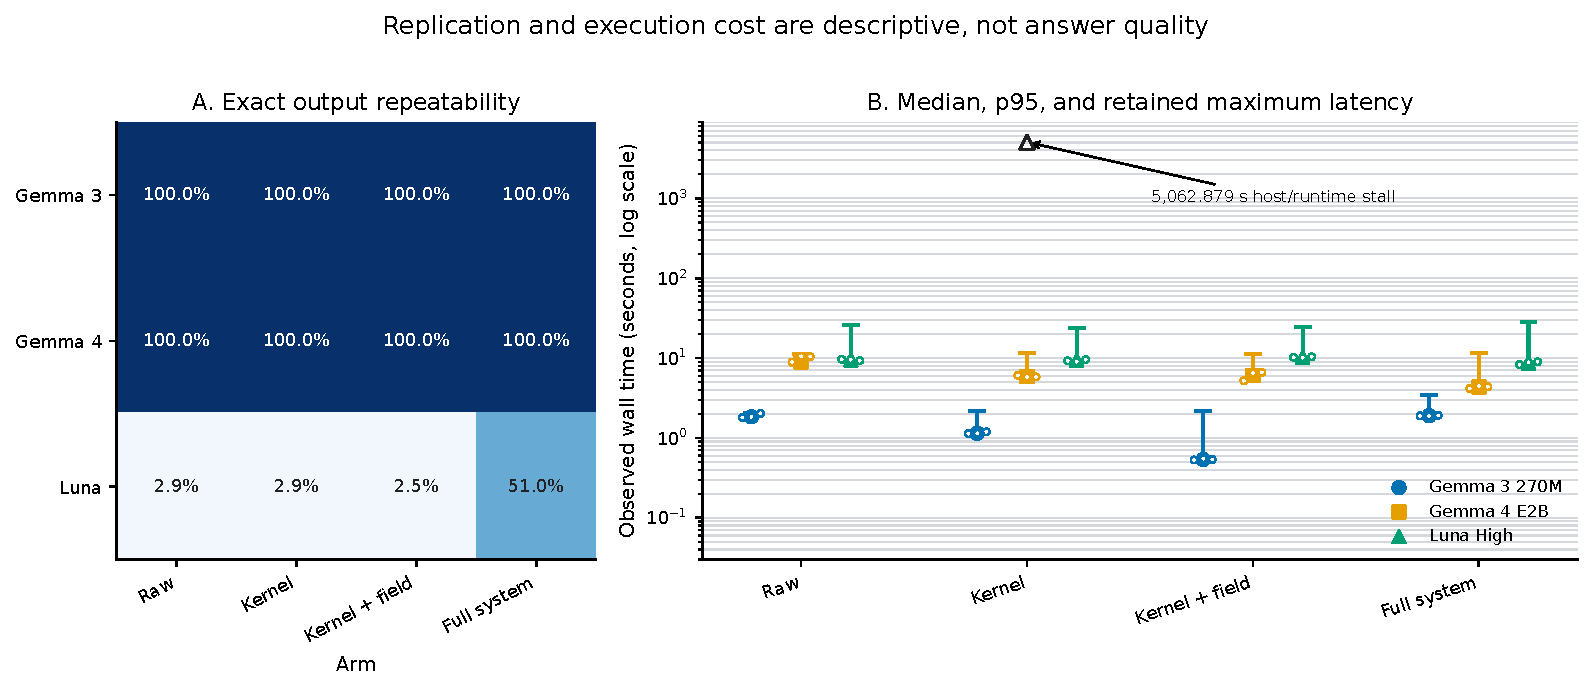
\includegraphics[width=0.98\textwidth]{figures/rc3_repeatability_latency.pdf}
  \caption{\textbf{Repeatability and observed execution time.} Exact output identity is correctness-neutral. Latency marks show overall median, p95, and per-trial medians on a logarithmic axis; the retained maximum identifies an unexplained host/runtime stall.}
  \label{fig:repeatability}
\end{figure*}

\section{Harness findings and repairs}

RC3 served as an adversarial test of the measurement system. The completed round exposed five material classes of defect:

\begin{enumerate}
  \item \textbf{Scorer semantics.} Correct generic product-mass units caused two false negatives. The accompanying release candidate includes a successor scorer that normalizes this unit only when the product-rate contract is explicit; RC3 remains unchanged.
  \item \textbf{Public metric naming.} The historical public-safe retention projection labelled lexical diagnostic values as \texttt{objective\_accuracy}. The accompanying release candidate includes a versioned successor that separates construct, rubric, diagnostic score, and objective accuracy. The nine frozen bundles remain verifiable.
  \item \textbf{Language preservation.} Three French Quebec cases ended in English deterministic authority holds, yielding 9/12 preservation. The accompanying release candidate includes a future-only language-aware policy renderer; the frozen failure remains reported.
  \item \textbf{Admission reporting.} A legacy aggregate called 22 explicit regional-context cases and 16 typed capability results ``weak retrieval.'' The accompanying release candidate includes a versioned report that separates these categories.
  \item \textbf{Routing and host diagnostics.} Expected local guards were complete on 134/154 eligible full-system cases, and one latency record contains an unexplained multi-thousand-second stall. Both remain investigation targets rather than silently filtered observations.
\end{enumerate}

The main scientific value of these findings is methodological: a benchmark harness should be one of the systems under test. Scoring, serialization, retention, identities, language routing, authorization, and reporting need adversarial controls just as retrieval and generation do.

\section{Limitations and next evidence}

RC3 is intentionally nonclaim. The exposed suite was inspected and used for repair. It has no real-user cases, no untouched prospective holdout, no independent agronomist judgments, no field outcomes, and no legal-compliance adjudication. Retrieval presence does not prove relevance or use. Verification activity does not prove improvement. Exact repetition does not prove correctness. Latency and token observations do not compare local energy with remote cost. Candidate configurations use different verification profiles, so cross-candidate full-system contrasts are not pure model effects.

Benchmark v3 should preserve the now-tested identity and retention boundary while adding: (1) an untouched, access-controlled prospective set; (2) independent two-phase agronomist review with calibrated adjudication; (3) a true component matrix with independently switchable document retrieval, graph retrieval, tools, answerability, and verification; (4) identical harness profiles where causal candidate comparison is intended; (5) preregistered endpoint families and promotion thresholds; and (6) explicit scenario-family identifiers for clustered uncertainty analysis. Service-orchestration and public-adapter behavior also remain outside RC3.

\section{Reproducibility and availability}

The public checkpoint includes answer-free response measurements, trial inventory, summary tables, four vector figures, exact generated manuscript values, a claim-to-evidence manifest, and a self-verifying package manifest. The analysis reads only the nine completion-receipted trial databases; it does not glob the retention root. It verifies database hashes, suite and source identities, arm and observation cardinalities, zero semantic judgments, the two frozen parser defects, the retained latency outlier, and all paired keys before producing a result. Machine-local paths are not serialized.

Raw answers, questions, prompts, context packets, SQLite databases, logs, model weights, and credentials are excluded from Git. They remain in separately controlled content-addressed bundles. The analysis source, public tables, and validation receipt support the reported aggregates and parser audit without exposing those private artifacts.

\section{Conclusion}

RC3 completed a demanding reproducibility exercise and materially strengthened \system{}. It demonstrates that the harness can execute and retain a full repeated matrix, bind local and remote paths to explicit identities, expose deterministic tools and authority holds, and surface defects in its own scoring and reporting. It does not yet tell us which candidate gives the best agronomic advice. That distinction is the honest result: RC3 provides a tested substrate for preserving and analyzing a future prospective benchmark, while answer-quality and field-reliability claims remain gated on independent evidence.

\paragraph{Competing interests.} No competing interests are declared.

\bibliographystyle{unsrtnat}
{\footnotesize\bibliography{references}}

\end{document}
